\begin{problem}{전단지 돌리기}{표준 입력(stdin)}{표준 출력(stdout)}{1\,초}{1024\,MB}

현민이는 트리 모양의 길 위에서 오토바이를 타고 전단지를 돌리려고 한다. 현민이의 목표는 케니소프트에서 출발하여 모든 노드에 전단지를 돌리고, 다시 케니소프트로 돌아오는 것이다. 현민이는 힘이 좋기 때문에 현재 노드에서 거리가 $D$ 이하인 모든 노드에 전단지를 돌릴 수 있다.

날씨가 매우 덥기 때문에, 현민이는 최소한만 이동해서 목표를 달성하고 싶다! 현민이를 위해 현민이가 이동해야 하는 총 거리를 구해주자.

\InputFile
첫번째 줄에는 노드의 개수 $N$($ 1 \leq N \leq 100\ 000 $)과 케니소프트의 위치 $S$($ 1 \leq S \leq N $), 힘 $D$($ 0 \leq D \leq N $)이 주어진다.

두 번째 줄부터 $N$번째 줄까지, 트리의 간선 정보를 의미하는 두 자연수 $x$, $y$가 공백으로 구분되어 주어진다. 이는 $x$번 노드와 $y$번 노드가 연결되어 있음을 의미한다. ($1 \leq x, y \leq N$, $x \neq y$)

주어지는 연결관계는 트리를 구성하며, 모든 간선의 길이는 $1$이다. 

\OutputFile
현민이가 목표를 완수하기 위해 이동해야 하는 최소 거리를 출력하여라.

\Example

\begin{example}
    \exmp{
        6 1 1
        1 2
        2 3
        2 4
        3 5
        5 6
    }{%
        6
    }%
\end{example}

\begin{figure}[h!]
\centering
  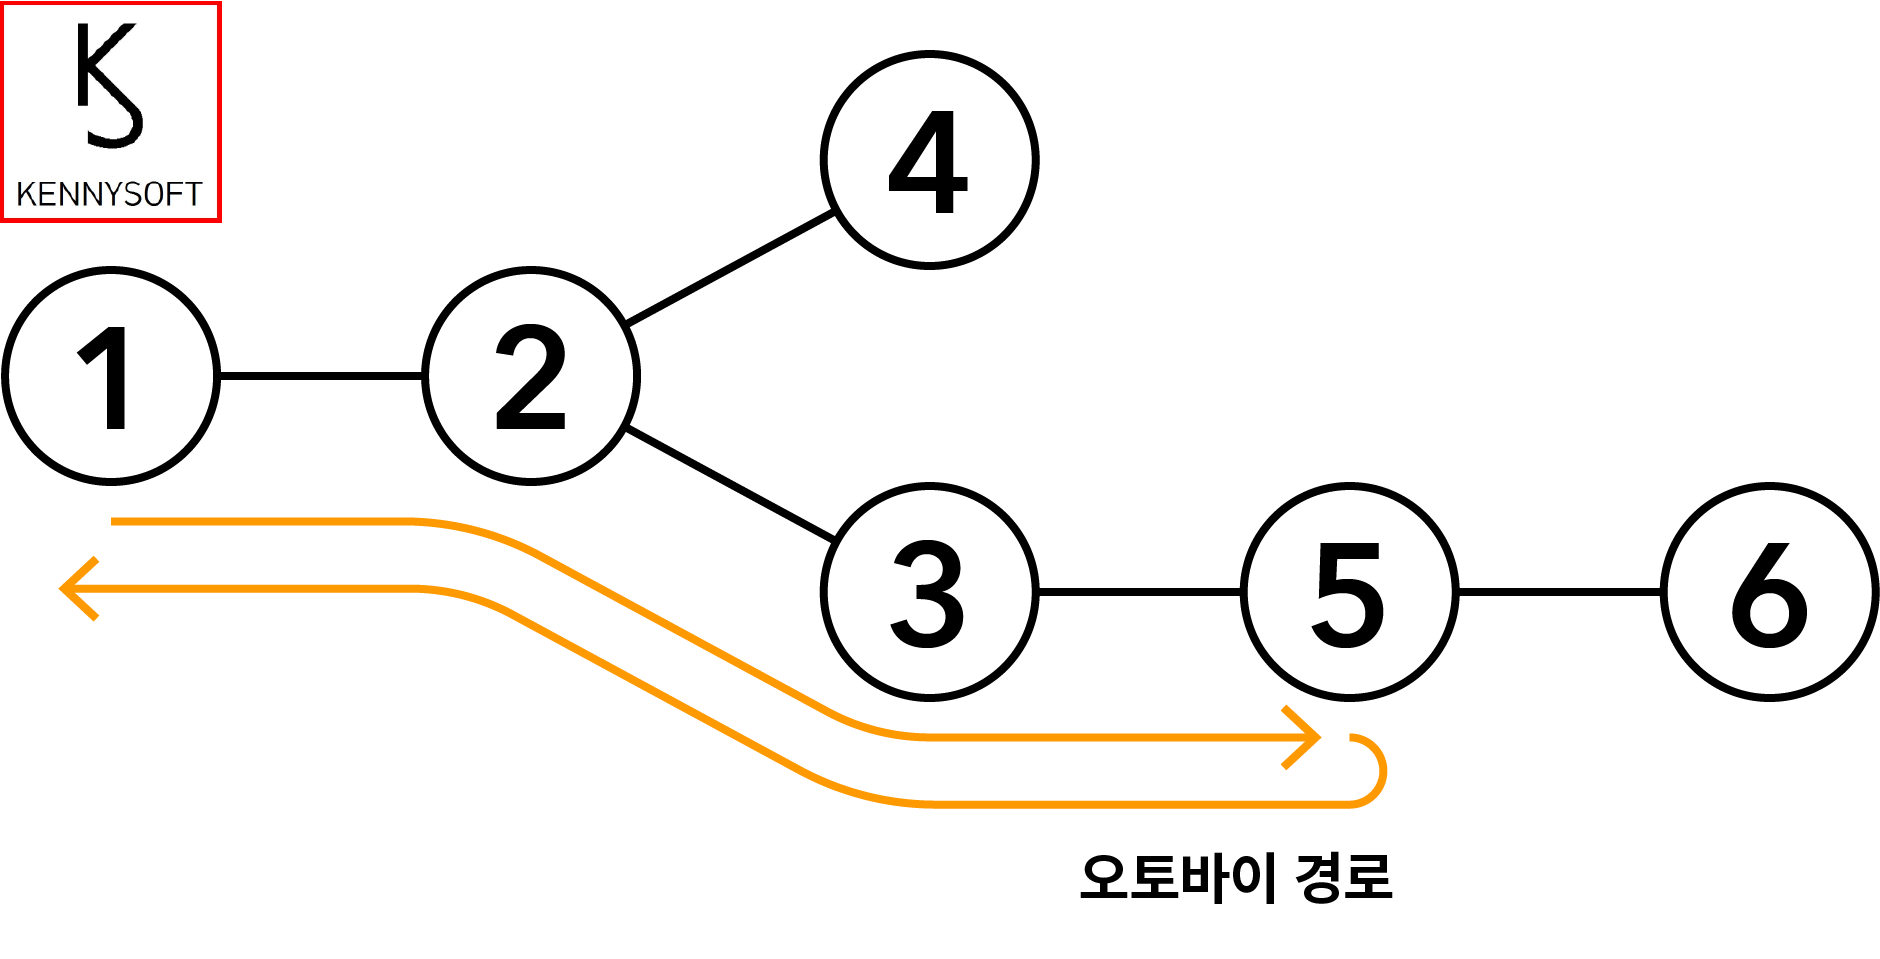
\includegraphics[width=.6\linewidth]{../pictures/leaflet@4x.png}
\end{figure}

\end{problem}